\section{Computational Experiment}

%TODO: The main section of the report. Describe and motivate the choice of tools and the distributed system that you designed. Describe how you have designed your scalability experiments,and present the results.

This section provides the motivation for our choice of tools and briefly describes the distributed system that we designed. 

\subsection{Tools \& Implementations}
We are using Spark as it provides a new model of computation that allows to perform multiple parallel operations on a specific set of data. In our project we apply multiple functions repeatedly to the same data set to extract various statistical information, hence Spark offers the possibility to improve significantly our performances without reloading each time the data form disk\cite{Sparkzaharia}.The thing which makes processing much faster in spark is because it runs on Memory(RAM).

Our dataset is spread among a read-only collection of objects called RDD, those objects allow parallel operations with the option of caching an RDD in memory so it can be reused for other MapReduce operations. An RDD does not exist in physical storage but it is computed from data in the reliable storage. 
We are constructing RDD from a \textit{.csv} file in a shared file system. The System we have is fault tolerant, in fact if a partition of an RDD is lost it is possible to rebuild just that partition given the information on how it was derived from other RDDs. This is called \textit{lineage}\cite{Sparkzaharia}.

In our system a \textit{driver program} connects to a cluster of \textit{workers}, these are processes that can store RDD partitions in RAM across operations\cite{RDD}.\newline
Our final code used pyspark RDD and dataframe for analyzing the dataset. We started to implement a working single node and tested so we could abstract the data we wanted. When this was working correctly, we implemented so we got a master node and 3 worker nodes.When we ran our code on 35 Gb dataset it divides the data in 288 partitions and computing them simultaneously on 3 nodes which makes the time taken for computation faster as you can see in Figure \ref{fig:stages_three_fourth}. We didn't tried but maybe increasing the number of partitions may improve the performance of our 3 node cluster. 

We created Virtual Machine at SNIC Science Cloud \cite{snic} and used the following settings:

\begin{itemize}
    \item \textbf{Source:} Volume Snapshot of 'snapshotgroup12'. We took the volume snapshot of master node which we configured for assignment 2 and increased its size to 40 GB and then used it for the project. This saved us a lot of time as we don't need to install everything from scratch.
    \item \textbf{Flavor:} $ssc.medium$ which had 2 VCPUs, 4Gb Ram, 40 Gb total disk and root disk
    \item \textbf{Networks:} SNIC 2018/10-13 Internal IPv4 Network.
    \item Our Cluster with 3 worker node has total of 6 cores(2 cores each) with the memory of 8.6 Gb(2.9 Gb each). You can see our Spark UI with 3 worker node in Figure \ref{fig:spark_master_three}. 
\end{itemize}

\begin{figure}[H]
    \centering
    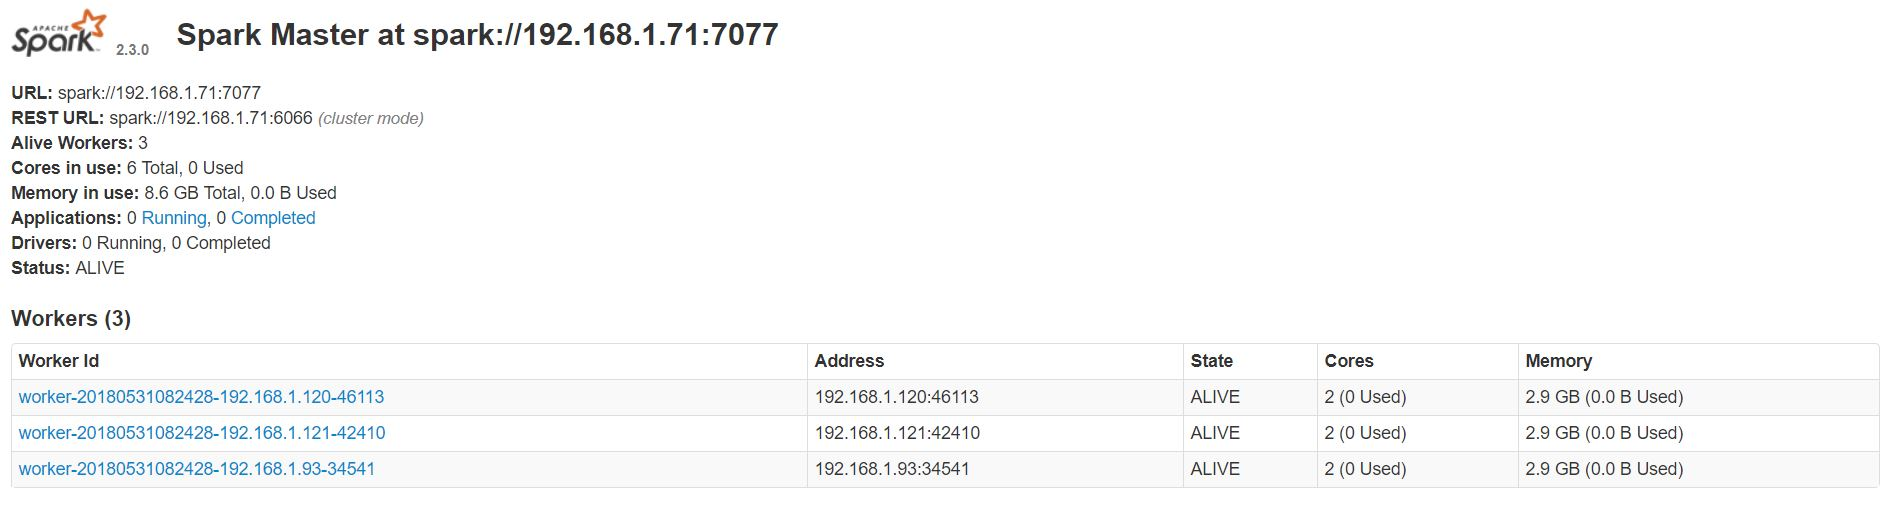
\includegraphics[width=.95\linewidth]{figures/spark_master_three.jpg}
    \caption{Screenshot of our Spark UI Cluster with 3 worker nodes.}
    \label{fig:spark_master_three}
\end{figure}


\subsection{Results}
For this project, we are using Crimes dataset\cite{cityOfChicago} from city of chicago portal and it contains many relevant information associated with each of the crime that has occurred in Chicago from year 2001 until now. We are plotting 4 different graphs associated with 4 different columns. A program in pyspark was created to plot these graph. You can look at the code \href{https://github.com/ankurshukla03/ldsaproject/blob/edit_report/code/Crimes.ipynb}{here.} \\
Below is 4 different plots presenting the results :\\

\mfigure{crime_type}{Plot representing the number of times a particular crime type has occured in Chicago from year 2001 until now. Our plot generated seems correct as you can check from Figure \ref{fig:exampleGraph} which we took from chicago portal \cite{cityOfChicago}.}

\mfigure{month}{Plot representing the frequency of crime across the months.}

\mfigure{year}{Plot representing the frequency of crime per year.}

\mfigure{location}{Plot repersenting the frequency of crime with location description. Our plot is correct when compared with the plot in the dashboard of chicago portal \href{https://data.cityofchicago.org/Public-Safety/Crimes-2001-to-present-Dashboard/5cd6-ry5g}{here.}}


\subsection{Scalability experiment}
In order to test and confirm the scalability of the system, scalability studies were conducted. Since the original dataset was only 1,45 GB, it was scaled up by replicating it in order to get larger datasets. Four different sizes of the dataset were produced including the original one. These were 1.45 Gb, 11.2 Gb, 23.2 Gb and 35 Gb and you can see the time taken with different number of nodes on these data size in Table \ref{table_time}.

To measure the horizontal scalability, the run time for a specific job on the dataset were recorded for 1 to 3 nodes in the cluster. As seen in  \ref{fig:scalabilityGraph} below we can observe that
the run time increased linearly with data size for the different cluster configurations and the run time was reduced equally for increasing number of nodes. Furthermore, the slopes for the linear fits of the data points are shown. The slope for one node is 41.241 s/GB and for four nodes it is 13.114 s/GB. This means that the second configuration is 3,15 times faster.\\

\begin{table}[]
    \centering
    \begin{tabular}{|c|c|c|}
\hline
Number of Nodes  & Time Taken & Data Size \\ \hline
        1 & 1.1 min & 1.45 Gb \\ \hline
        3 & 32 seconds & 1.45 Gb \\
\hline
\end{tabular}
\quad
\begin{tabular}{|c|c|c|}
\hline
Number of Nodes  & Time Taken & Data Size \\ \hline
        1 & 4.1 min & 5.8 Gb \\ \hline
        3 & 1.4 min & 5.8 Gb \\
\hline
\end{tabular}
\begin{tabular}{|c|c|c|}
\hline
Number of Nodes  & Time Taken & Data Size \\ \hline
        1 & 16 min & 23.2 Gb \\ \hline
        3 & 5.1 min & 23.2 Gb \\
\hline
\end{tabular}
\quad
\begin{tabular}{|c|c|c|}
\hline
Number of Nodes  & Time Taken & Data Size \\ \hline
        1 & 24 min & 35 Gb \\ \hline
        3 & 7.6 min & 35 Gb \\
\hline
\end{tabular}
    \caption{Time taken by different number of nodes on different data size. We are writing here only the time taken by reduce functionality as it is so large compare to other functions that it has a significant role while computing time taken by our code as you can see in figure \ref{fig:stages_one_fourth}.}
    \label{table_time}
\end{table}


\mfigure{stages_one_fourth}{Screenshot of our Spark UI stages tab when ran with 1 node on 35 Gb data size.}

\mfigure{stages_three_second}{Screenshot of our Spark UI stages tab when ran with 3 node on 5.8 Gb data size.}

\mfigure{stages_three_fourth}{Screenshot of our Spark UI stages tab when ran with 3 worker node on 35 Gb data size.}


\begin{figure}[H]
    \centering
    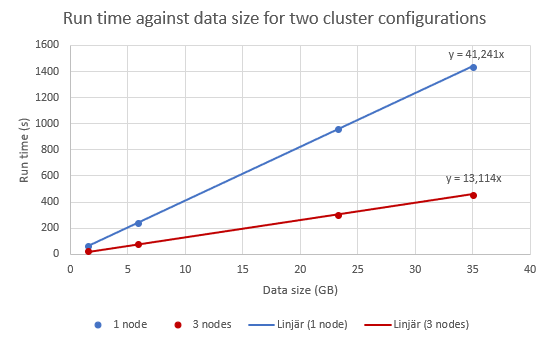
\includegraphics[width=.75\linewidth]{figures/runTime2.PNG}
    \caption{Run time for different data sizes plotted for two cluster configurations. Blue line is the cluster with one node and the red line is with three nodes.}
    \label{fig:scalabilityGraph}
\end{figure}

